\begin{center}
	\Huge
	Differentialligninger i Maple
\end{center}

\section*{Differentialligninger i Maple}
\stepcounter{section}
Vi skal i dag se, hvordan vi løser differentialligninger i Maple. Dette er lidt kompliceret, da syntaksen i kommandoen godt kan være lidt besværlig.

\begin{exa}
	Vi får givet en differentialligning
	\begin{align*}
		\frac{dy}{dx} = \frac{y}{x^2}.
	\end{align*}
	Vi begynder med at finde en fuldstændig løsning til differentialligningen. Dette gøres i Maple ved kommandoen 
	\texttt{dsolve}.


	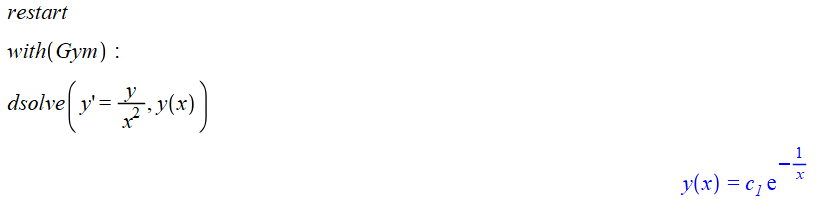
\includegraphics[width=1\textwidth]{Billeder/dsolve}
	
	Vi får altså løsningen
	\begin{align*}
		y(x) = ce^{-\frac{1}{x}}.
	\end{align*}
	
	Når man løser differentialligninger i Maple, skriver man først sin differentialligning, altså 
	\begin{align*}
		y' = \frac{y}{x^2}
	\end{align*}
	og dernæst den løsning, man ønsker, altså $y(x)$.
	Vi kan også finde en partikulær løsning. Vi betragter derfor det tilfælde, at vi har fået bibetingelsen $y(2) = 5$.
	

	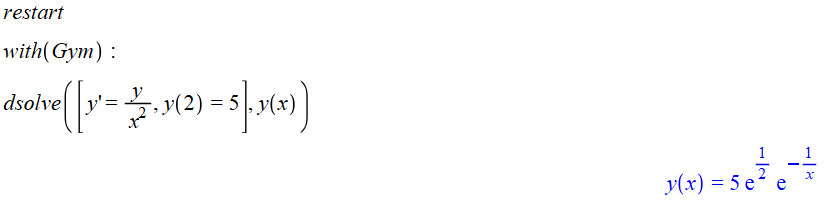
\includegraphics[width = 1\textwidth]{Billeder/dsolve2}

	Dette giver os løsningen
	\begin{align*}
		y(x) = 5e^\frac{1}{2}e^{-\frac{1}{x}}
	\end{align*}
	Når vi finder løsninger med bibetingelser, skriver vi altså først en liste med ligningen og bibetingelsen, her
	\begin{align*}
		\left[ y' = \frac{y}{x^2}, y(2) = 5\right]
	\end{align*}
	Efterfølgende opskriver vi vores ønskede funktion som før, altså $y(x)$. 
\end{exa}

\newpage

\subsection*{Opgave 1 (Med hjælpemidler)}
En differentialligning er givet ved
\begin{align*}
	y' = 10y - xy.
\end{align*}
\begin{enumerate}[label=\roman*)]
	\item Bestem en fuldstændig løsning til differentialligningen.
	\item Bestem en partikulær løsning til differentialligningen, der går gennem punktet $(0, 10)$. 
\end{enumerate}


\subsection*{Opgave 2 (Med hjælpemidler)}
En differentialligning er givet ved
\begin{align*}
	y' = 3xy - 2y.
\end{align*}
\begin{enumerate}[label=\roman*)]
	\item Bestem en fuldstændig løsning til differentialligningen.
	\item Bestem en partikulær løsning til differentialligningen, der går gennem punktet $(1, 5)$.
\end{enumerate}



\subsection*{Opgave 3 (Med hjælpemidler)}
En kop kaffe har temperaturen $90\ ^{\circ}$C, når den hældes op. Temperaturen i lokalet er konstant $20\ ^{\circ}$C. I en model beskrives kaffens temperatur $T(t)$ ved differentialligningen
\begin{align*}
	T'(t) = -0.08\left(T(t)-20\right),
\end{align*}
hvor $t$ er tiden i minutter efter ophældningen, og $T(t)$ måles i grader Celsius.
\begin{enumerate}[label=\roman*)]
	\item Bestem ved hjælp af Maple en forskrift for $T(t)$, når $T(0)=90$.
	\item Brug løsningen til at bestemme kaffens temperatur efter 10 minutter.
	\item Kaffen er drikkeklar, når temperaturen er højst $60\,^{\circ}\mathrm{C}$. Hvor længe skal man ifølge modellen mindst vente?
\end{enumerate}

\subsection*{Opgave 4 (Med hjælpemidler)}
I et forsøg undersøges væksten af en bakteriekultur. Ved forsøgets begyndelse er der 500 bakterier. I en model beskrives antallet $N(t)$ ved differentialligningen
\begin{align*}
	N'(t) = 0.6N(t),
\end{align*}
hvor $t$ er tiden i timer efter forsøgets begyndelse. Modellen antages at gælde i de første 6 timer.
\begin{enumerate}[label=\roman*)]
	\item Bestem ved hjælp af Maple en forskrift for $N(t)$, når $N(0)=500$.
	\item Brug løsningen til at bestemme antallet af bakterier efter 4 timer.
	\item En ny måling skal foretages, når antallet af bakterier når 5000. Bestem ud fra løsningen, hvornår målingen skal foretages.
\end{enumerate}

\subsection*{Opgave 5 (Med hjælpemidler)}
En tank indeholder 100 liter rent vand. Saltvand med en koncentration på $2$ gram salt pr. liter ledes ind i tanken med $5$ liter pr. minut. Samtidig løber $5$ liter af tankens væske ud pr. minut. Det antages, at saltet fordeles jævnt ud i væsken. 

I en model beskrives saltmængden $S(t)$ i tanken ved differentialligningen
\begin{align*}
	S'(t) = 10-0.05S(t),
\end{align*}
hvor $t$ er tiden i minutter efter tilførslen starter, og $S(t)$ måles i gram.
\begin{enumerate}[label=\roman*)]
	\item Bestem ved hjælp af Maple en forskrift for $S(t)$, når $S(0)=0$.
	\item Brug løsningen til at bestemme saltmængden efter 20 minutter, og beregn saltkoncentrationen i tanken på dette tidspunkt.
	\item Bestem, hvornår saltkoncentrationen i tanken når $1.5$ gram pr. liter.
\end{enumerate}

\subsection*{Opgave 6 (Med hjælpemidler)}

En person er på hospitalet behandlet med et lægemiddel, og der tages løbende prøver for at måle koncentrationen af lægemiddelet. Både koncentrationen og nedbrydningshastigheden måles.  
Resultatet af målingerne fremgår af Tabel \ref{tab:medicin}. 
\begin{table}[H]
	\centering
	\rowcolors{1}{SeaGreen!70}{SeaGreen!30}
	\begin{tabular}{cccccccc}
		Koncentration $(y)$ & 103.1 & 99.5 & 95.7 & 92.3 & 88.6 & 85.2 & 81.1 \\
		Nedbrydningshastighed $(y')$ & $-2.02$ & $-1.96$ & $-1.90$ & $-1.83$ & $-1.75$ & $-1.69$ & $-1.61$ 
	\end{tabular}
	\caption{Oversigt over koncentration og nedbrydningshastighed.}
	\label{tab:medicin}
\end{table}

Det antages, at sammenhængen mellem nedbrydningshastigheden $y'$ og koncentrationen $y$ kan beskrives ved en sammenhæng af typen
\begin{align*}
	y' = ky,
\end{align*}
hvor koncentrationen $y$ er i milligram per liter $\left(\frac{\textnormal{mg}}{\textnormal{L}}\right)$ og nedbrydningshastigheden $y'$ er i milligram per liter per time $\left(\frac{\textnormal{mg}}{\textnormal{L}\cdot \textnormal{s}}\right)$
\begin{enumerate}[label=\roman*)]
	\item Bestem tallet $k$ ved hjælp af lineær regression. 
	\item Find en løsning til differentialligningen, hvis det oplyses, at koncentrationen til tidspunktet $t = 0$ er 110 mg/L.
	\item Bestem koncentrationen af lægemiddel efter 24 timer.
	\item Bestem det tidspunkt, hvor koncentrationen af lægemiddelet er halveret. 
\end{enumerate}

\subsection*{Opgave 7 (Med hjælpemidler)}

I en by kan antallet af beboere beskrives ved en differentialligning af typen
\begin{align*}
	\frac{dy}{dt} = 0.0046\cdot y \cdot (15 - y),
\end{align*}
hvor $y$ er antallet af personer i byen i mio. og $t$ betegner antal år siden år 2005.
\begin{enumerate}[label=\roman*)]
	\item Bestem en partikulær løsning til differentialligningen, hvis det oplyses, at antallet af personer i byen i år 2005 var 5.1 mio. 
	\item Tegn grafen for løsningen på intervallet $x \in [0, 80]$. 
	\item Bestem det år, hvor befolkningen i byen vokser hurtigst. 
\end{enumerate}

